\chapter{BULGULAR VE TARTIŞMA}

\section{Tek-Model Kanıtı (Profiling ve Gecikme)}
Şekil~\ref{fig:perf-compare}, tek-model benchmark koşusunda baseline ve optimized ortalama gecikme değerlerini özetler.
Grafik optimizasyonları düğüm sayısını azaltsa bile uçtan uca gecikme; sağlayıcı derleme ek yükü, kernel seçimi değişimi veya bellek-sınırlı davranış gibi nedenlerle artabilir.

\begin{figure}[h!]
	\centering
	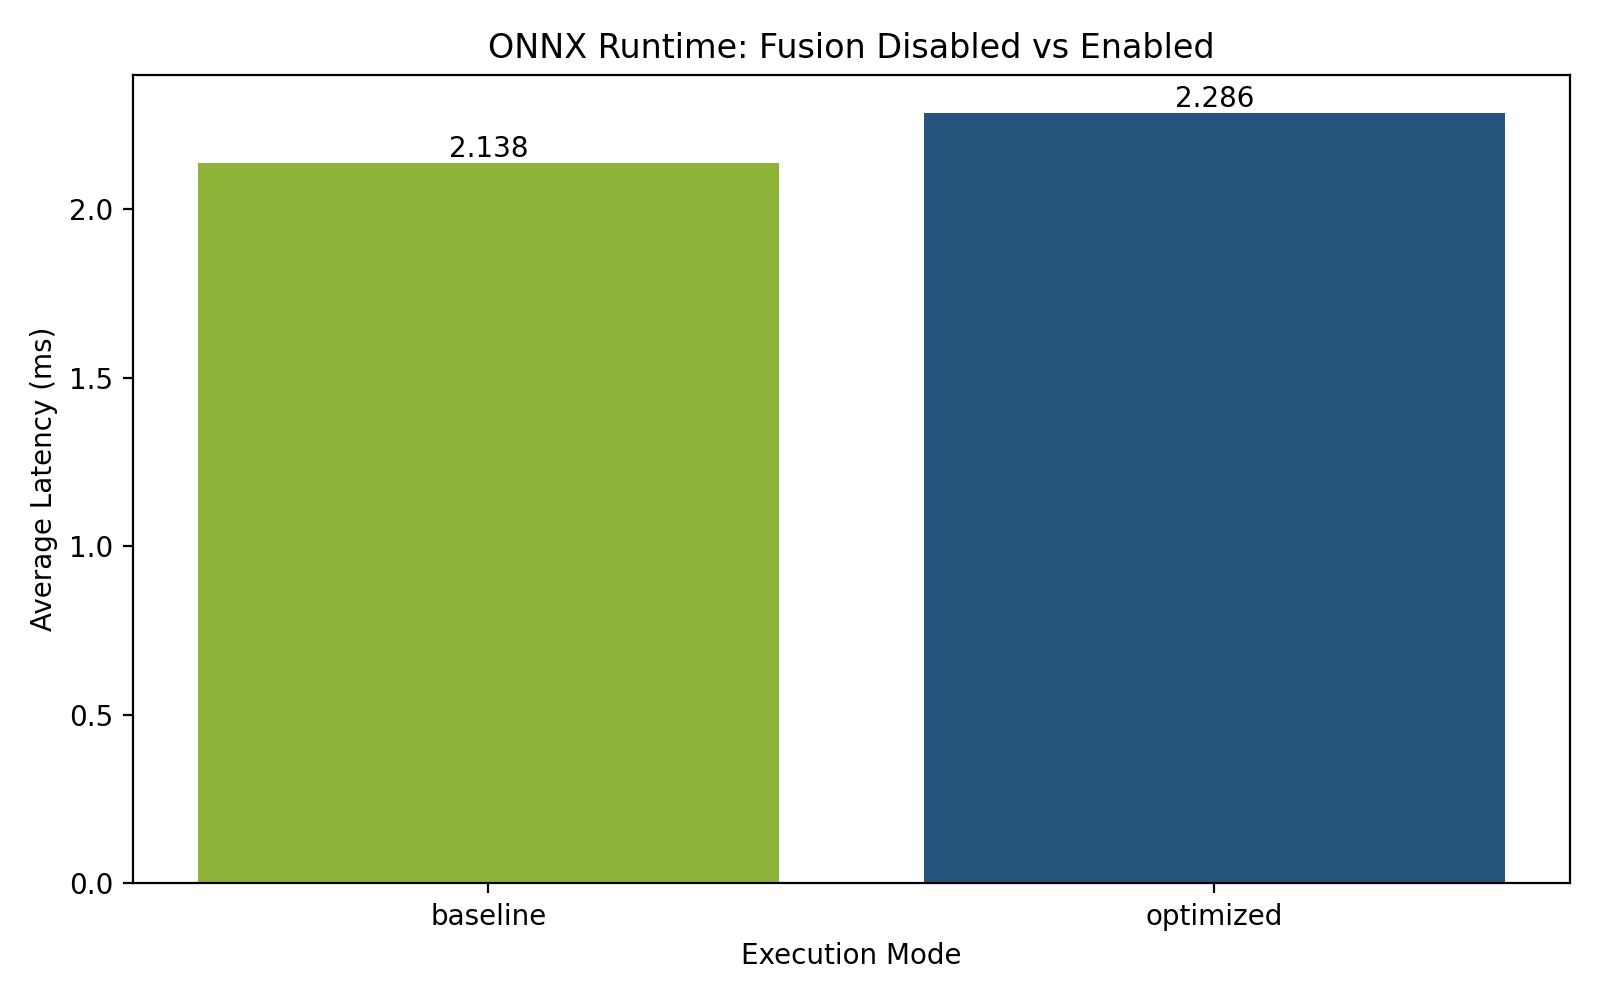
\includegraphics[width=0.95\linewidth]{figures/performance_comparison.png}
	\caption{Baseline ve optimized ortalama gecikme (ms).}
	\label{fig:perf-compare}
\end{figure}

Operatör-seviyesi kırılımlar, çalışma zamanını hangi operatörlerin domine ettiğine dair daha ince kanıt sağlar.
Şekil~\ref{fig:op-breakdown}, top-k operatör süre dağılımını göstermektedir.

\begin{figure}[h!]
	\centering
	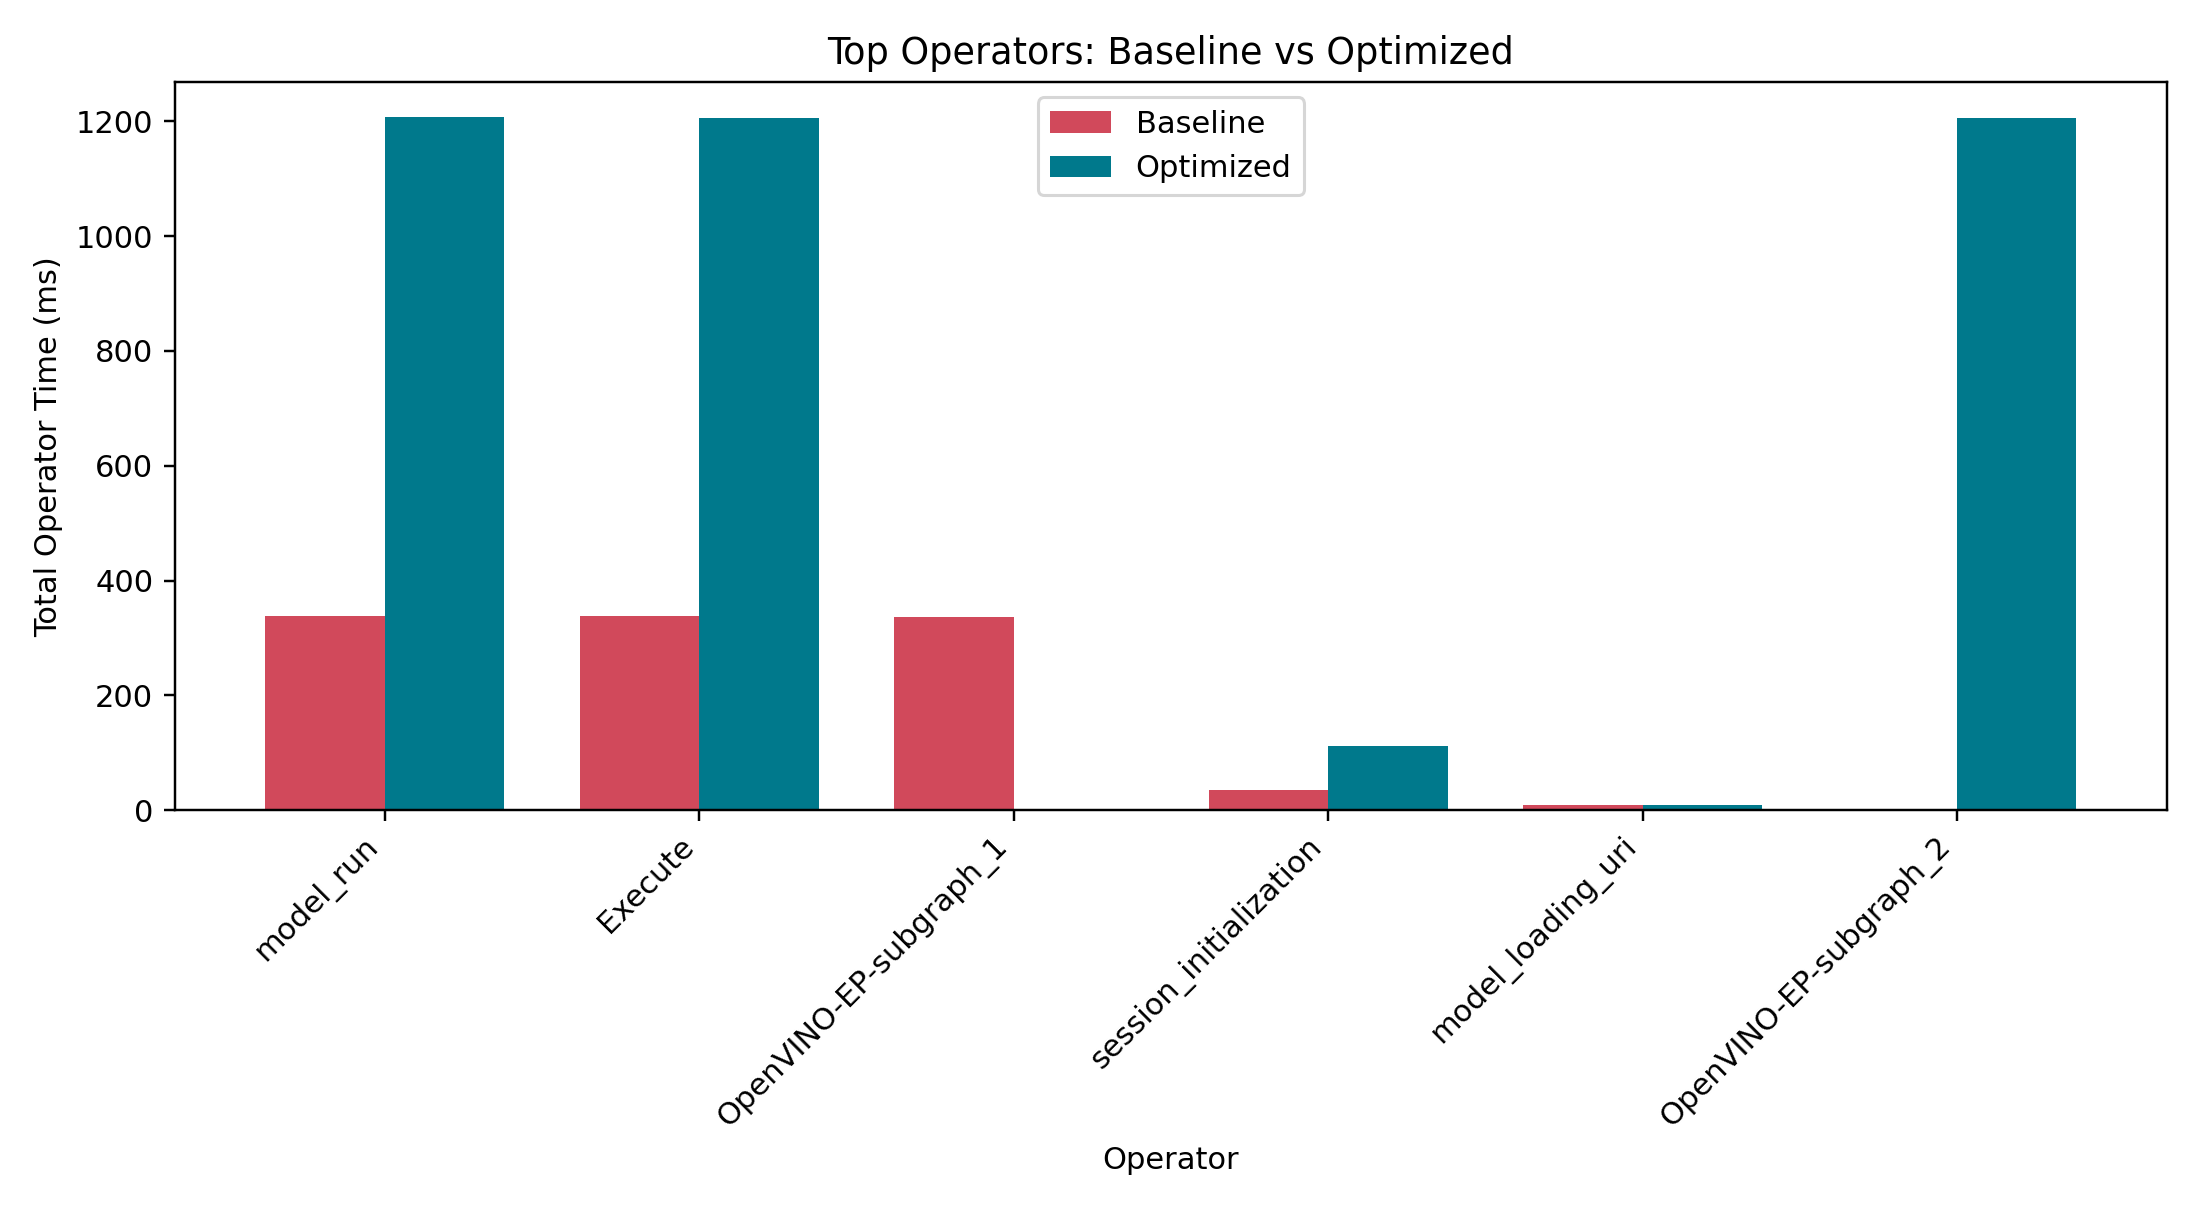
\includegraphics[width=0.95\linewidth]{figures/operator_breakdown_topk.png}
	\caption{Top-k operatör süre kırılımı (baseline vs optimized).}
	\label{fig:op-breakdown}
\end{figure}

\section{Çoklu Model Ölçeklenebilirliği}
Sonraki adımda üç model karşılaştırılarak düğüm azalımı ile gecikme etkisinin model ölçeğiyle nasıl değiştiği incelenmiştir.
Şekil~\ref{fig:scal-speedup} hızlanma oranını (baseline/optimized), Şekil~\ref{fig:scal-lat} ise mutlak gecikmeyi göstermektedir.

\begin{figure}[h!]
	\centering
	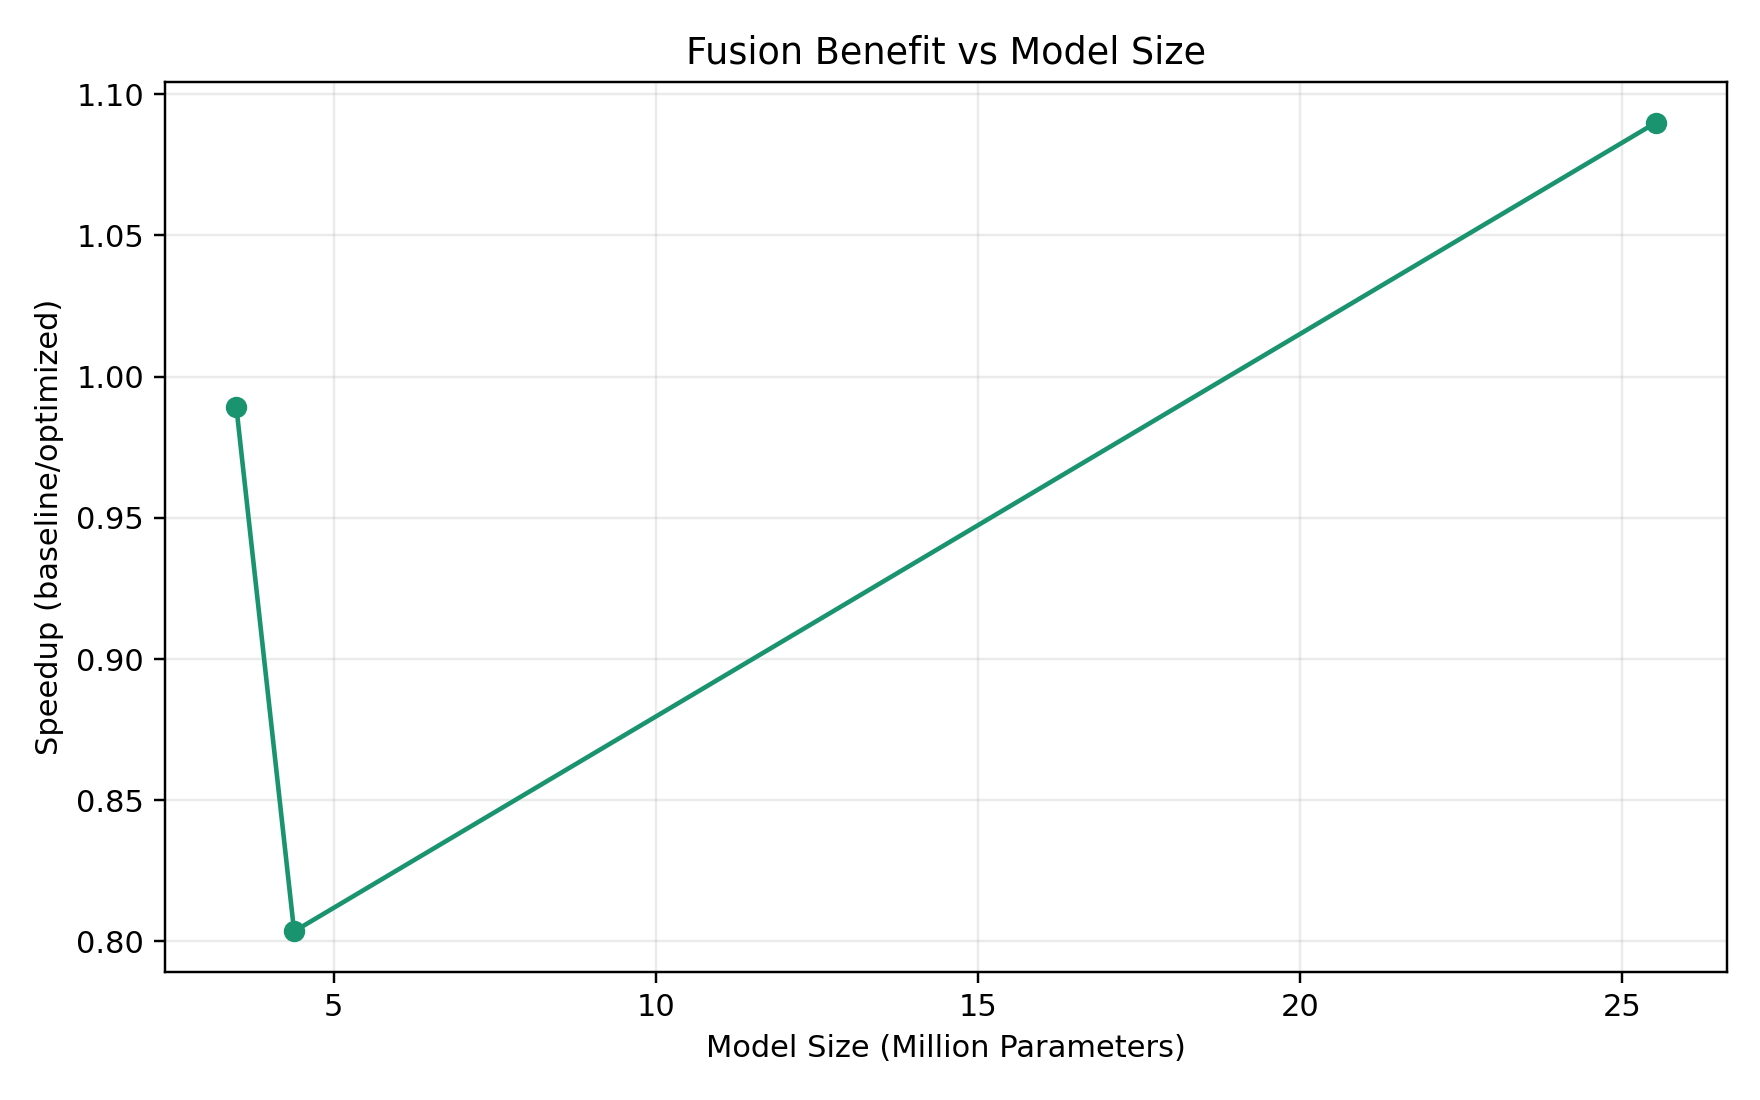
\includegraphics[width=0.95\linewidth]{figures/scalability_speedup.png}
	\caption{Modeller arası hızlanma (baseline/optimized).}
	\label{fig:scal-speedup}
\end{figure}

\begin{figure}[h!]
	\centering
	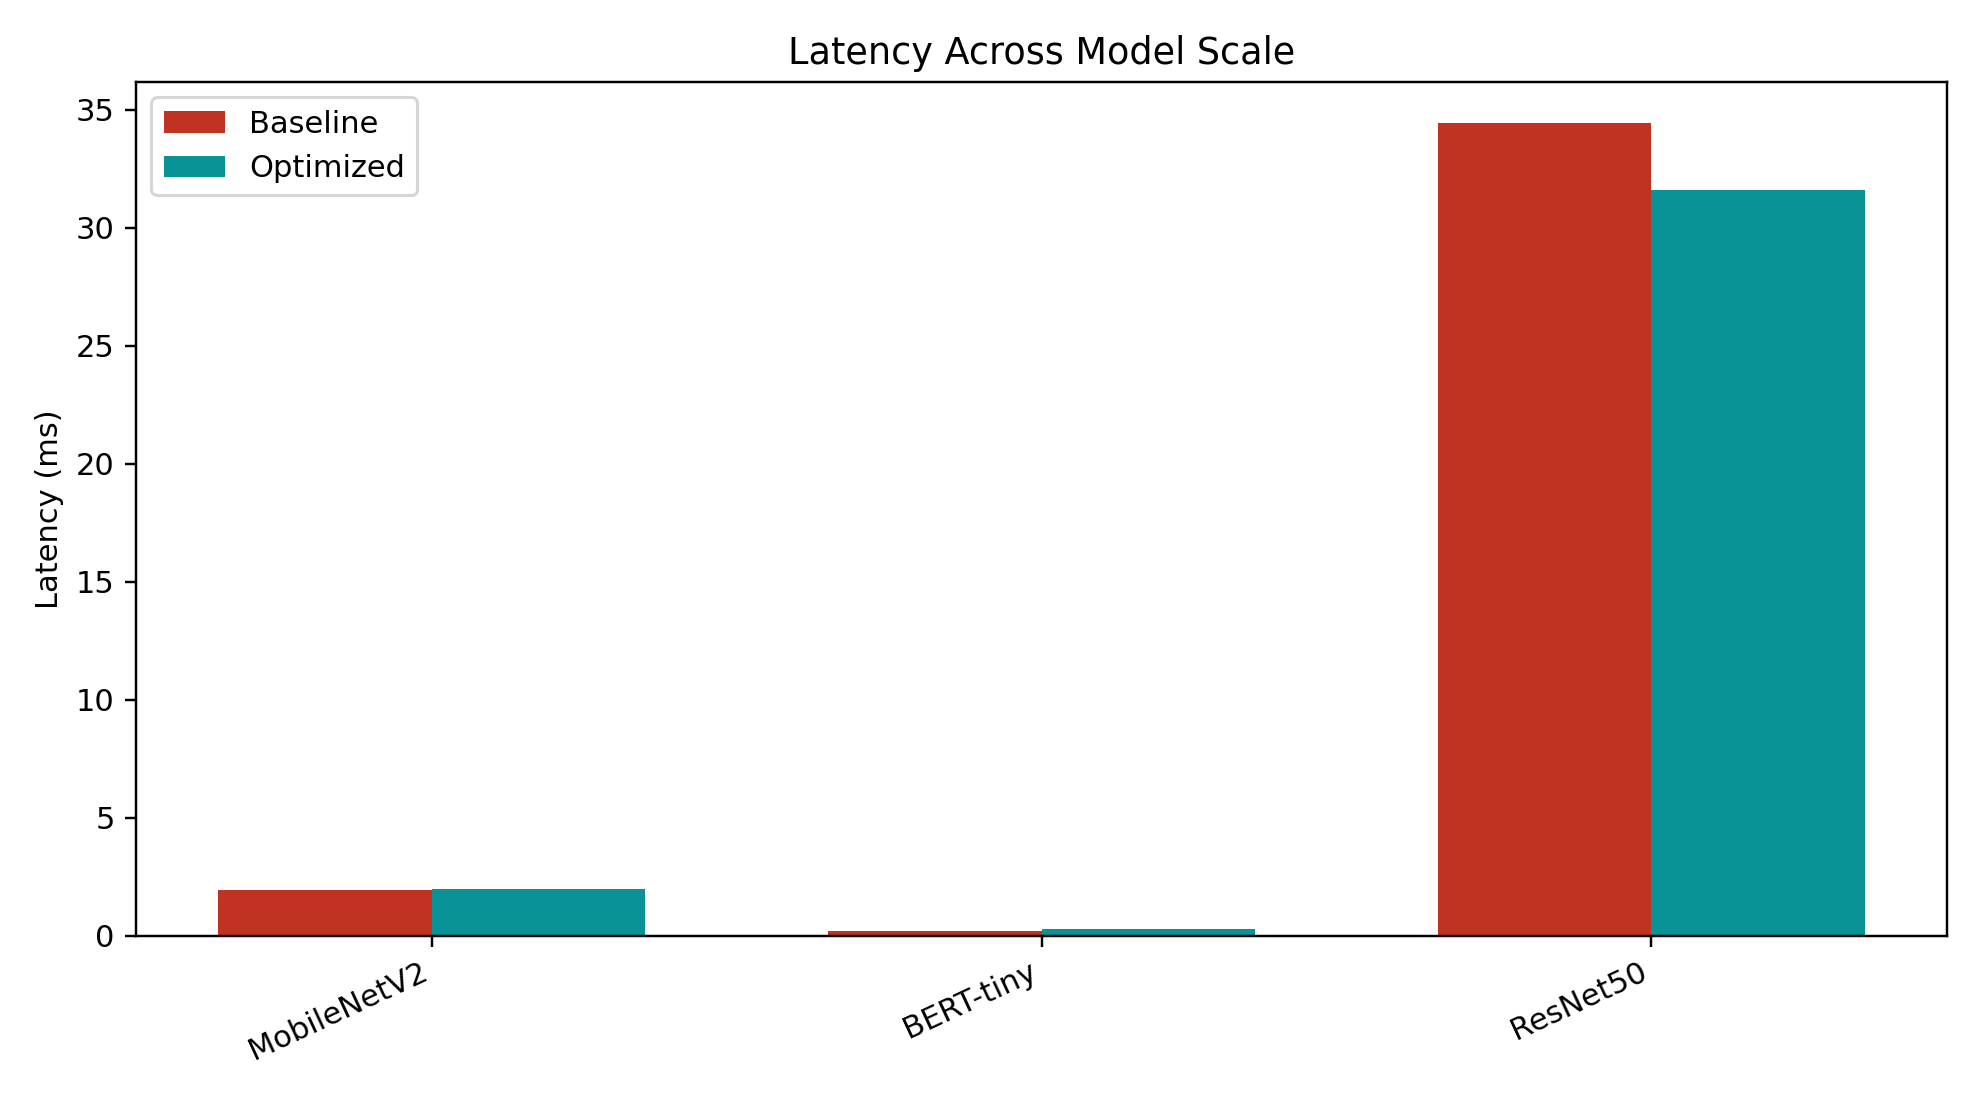
\includegraphics[width=0.95\linewidth]{figures/scalability_latency.png}
	\caption{Modeller arası gecikme (ms).}
	\label{fig:scal-lat}
\end{figure}

\section{Özet Tablo}
Tablo~\ref{tab:scalability}, \texttt{results/scalability\_matrix.csv} dosyasından çıkarılan temel metrikleri özetler.

\begin{table}[h!]
\centering
\caption{Çoklu model özeti (ortalama gecikme ve düğüm azalımı).}
\label{tab:scalability}
\begin{tabular}{lrrrrr}
\hline
\textbf{Model} & \textbf{Nodes} & \textbf{Opt. Nodes} & \textbf{Node Red. (\%)} & \textbf{Base (ms)} & \textbf{Opt. (ms)} \\
\hline
MobileNetV2 & 100 & 65 & 35.00 & 1.943 & 1.964 \\
BERT-tiny  & 233 & 74 & 68.24 & 0.213 & 0.265 \\
ResNet50   & 125 & 91 & 27.20 & 34.442 & 31.599 \\
\hline
\end{tabular}
\end{table}

\section{Tartışma}
İki gözlem öne çıkmaktadır.
Birincisi, düğüm azalımı yapısal bir metriktir ve doğrudan gecikme azalımı anlamına gelmez.
İkincisi, etki modele bağlıdır: ölçülen koşularda MobileNetV2 ve BERT-tiny küçük bir regresyon gösterirken ResNet50 iyileşmiştir.
Bu durum, füzyon ve grafik yeniden yazımlarının EP davranışı, derleme maliyeti ve bellek-sınırlı çalışma bağlamında değerlendirilmesi gerektiğini destekler \cite{memorywall}.